\documentclass[12pt]{article}
\usepackage{hyperref}
\usepackage{listings}
\usepackage[margin=1in]{geometry}
\usepackage{enumitem}
\usepackage{multicol}
\usepackage{array}
\usepackage{titlesec}
\usepackage{helvet}
\renewcommand{\familydefault}{\sfdefault}
\usepackage{amsmath}     % For math equations
\usepackage{amssymb}     % For advanced math symbols
\usepackage{amsfonts} % For math fonts
\usepackage{gvv}
\usepackage{esint}
\usepackage[utf8]{inputenc}
\usepackage{graphicx}
\usepackage{pgfplots}
\pgfplotsset{compat=1.18}
\titleformat{\section}{\bfseries\large}{\thesection.}{1em}{}
\setlength{\parindent}{0pt}
\setlength{\parskip}{6pt}
\usepackage{multirow}
\usepackage{float}
\usepackage{caption}


\begin{document}

\noindent\textbf{Problem 2.10.21 :}  
Let $\vec{a}$ and $\vec{b}$ be two non-collinear unit vectors. If  
\begin{align}
\vec{u} = \vec{a} - (\vec{a}\cdot \vec{b})\vec{b}, 
\quad 
\vec{v} = \vec{a} \times \vec{b},
\end{align}
find $\|\vec{v}\|$.


\text{(a)}\; $\|\vec{u}\|$ \\
\text{(b)}\; $\|\vec{u}\| + |\vec{u}\cdot \vec{a}|$ \\
\text{(c)}\; $\|\vec{u}\| + |\vec{u}\cdot \vec{b}|$ \\
\text{(d)}\; $\|\vec{u}\| + \vec{u}\cdot(\vec{a}+\vec{b})$



\textbf{Solution}

\begin{align}
\|\vec{u}\|^2 
&= \vec{u}^T \vec{u} \notag \\
&= \big(\vec{a} - (\vec{a}\cdot\vec{b})\vec{b}\big)^T 
   \big(\vec{a} - (\vec{a}\cdot\vec{b})\vec{b}\big) \notag \\
&= \vec{a}^T\vec{a} - 2(\vec{a}\cdot\vec{b})^2 + (\vec{a}\cdot\vec{b})^2 \,\vec{b}^T\vec{b} \notag \\
&= \|\vec{a}\|^2 - (\vec{a}\cdot\vec{b})^2 
   \qquad (\text{since }\|\vec{a}\|=\|\vec{b}\|=1) \notag \\
&= 1 - (\vec{a}\cdot\vec{b})^2.
\end{align}

\begin{align}
\|\vec{v}\|^2 
&= \|\vec{a}\times\vec{b}\|^2 \notag \\
&= \|\vec{a}\|^2 \|\vec{b}\|^2 - (\vec{a}\cdot\vec{b})^2 
   \qquad (\text{vector identity}) \notag \\
&= 1 - (\vec{a}\cdot\vec{b})^2. 
\end{align}

\begin{align}
(2) \text{ and } (3) \;\;\implies\;\;
\|\vec{v}\|^2 = \|\vec{u}\|^2 
&\;\;\;\Rightarrow\;\;\; 
\|\vec{v}\| = \|\vec{u}\|.
\end{align}

\begin{align}
\boxed{\|\vec{v}\| = \|\vec{u}\|}
\end{align}

Option A is correct

\begin{figure}[H]
    \centering
    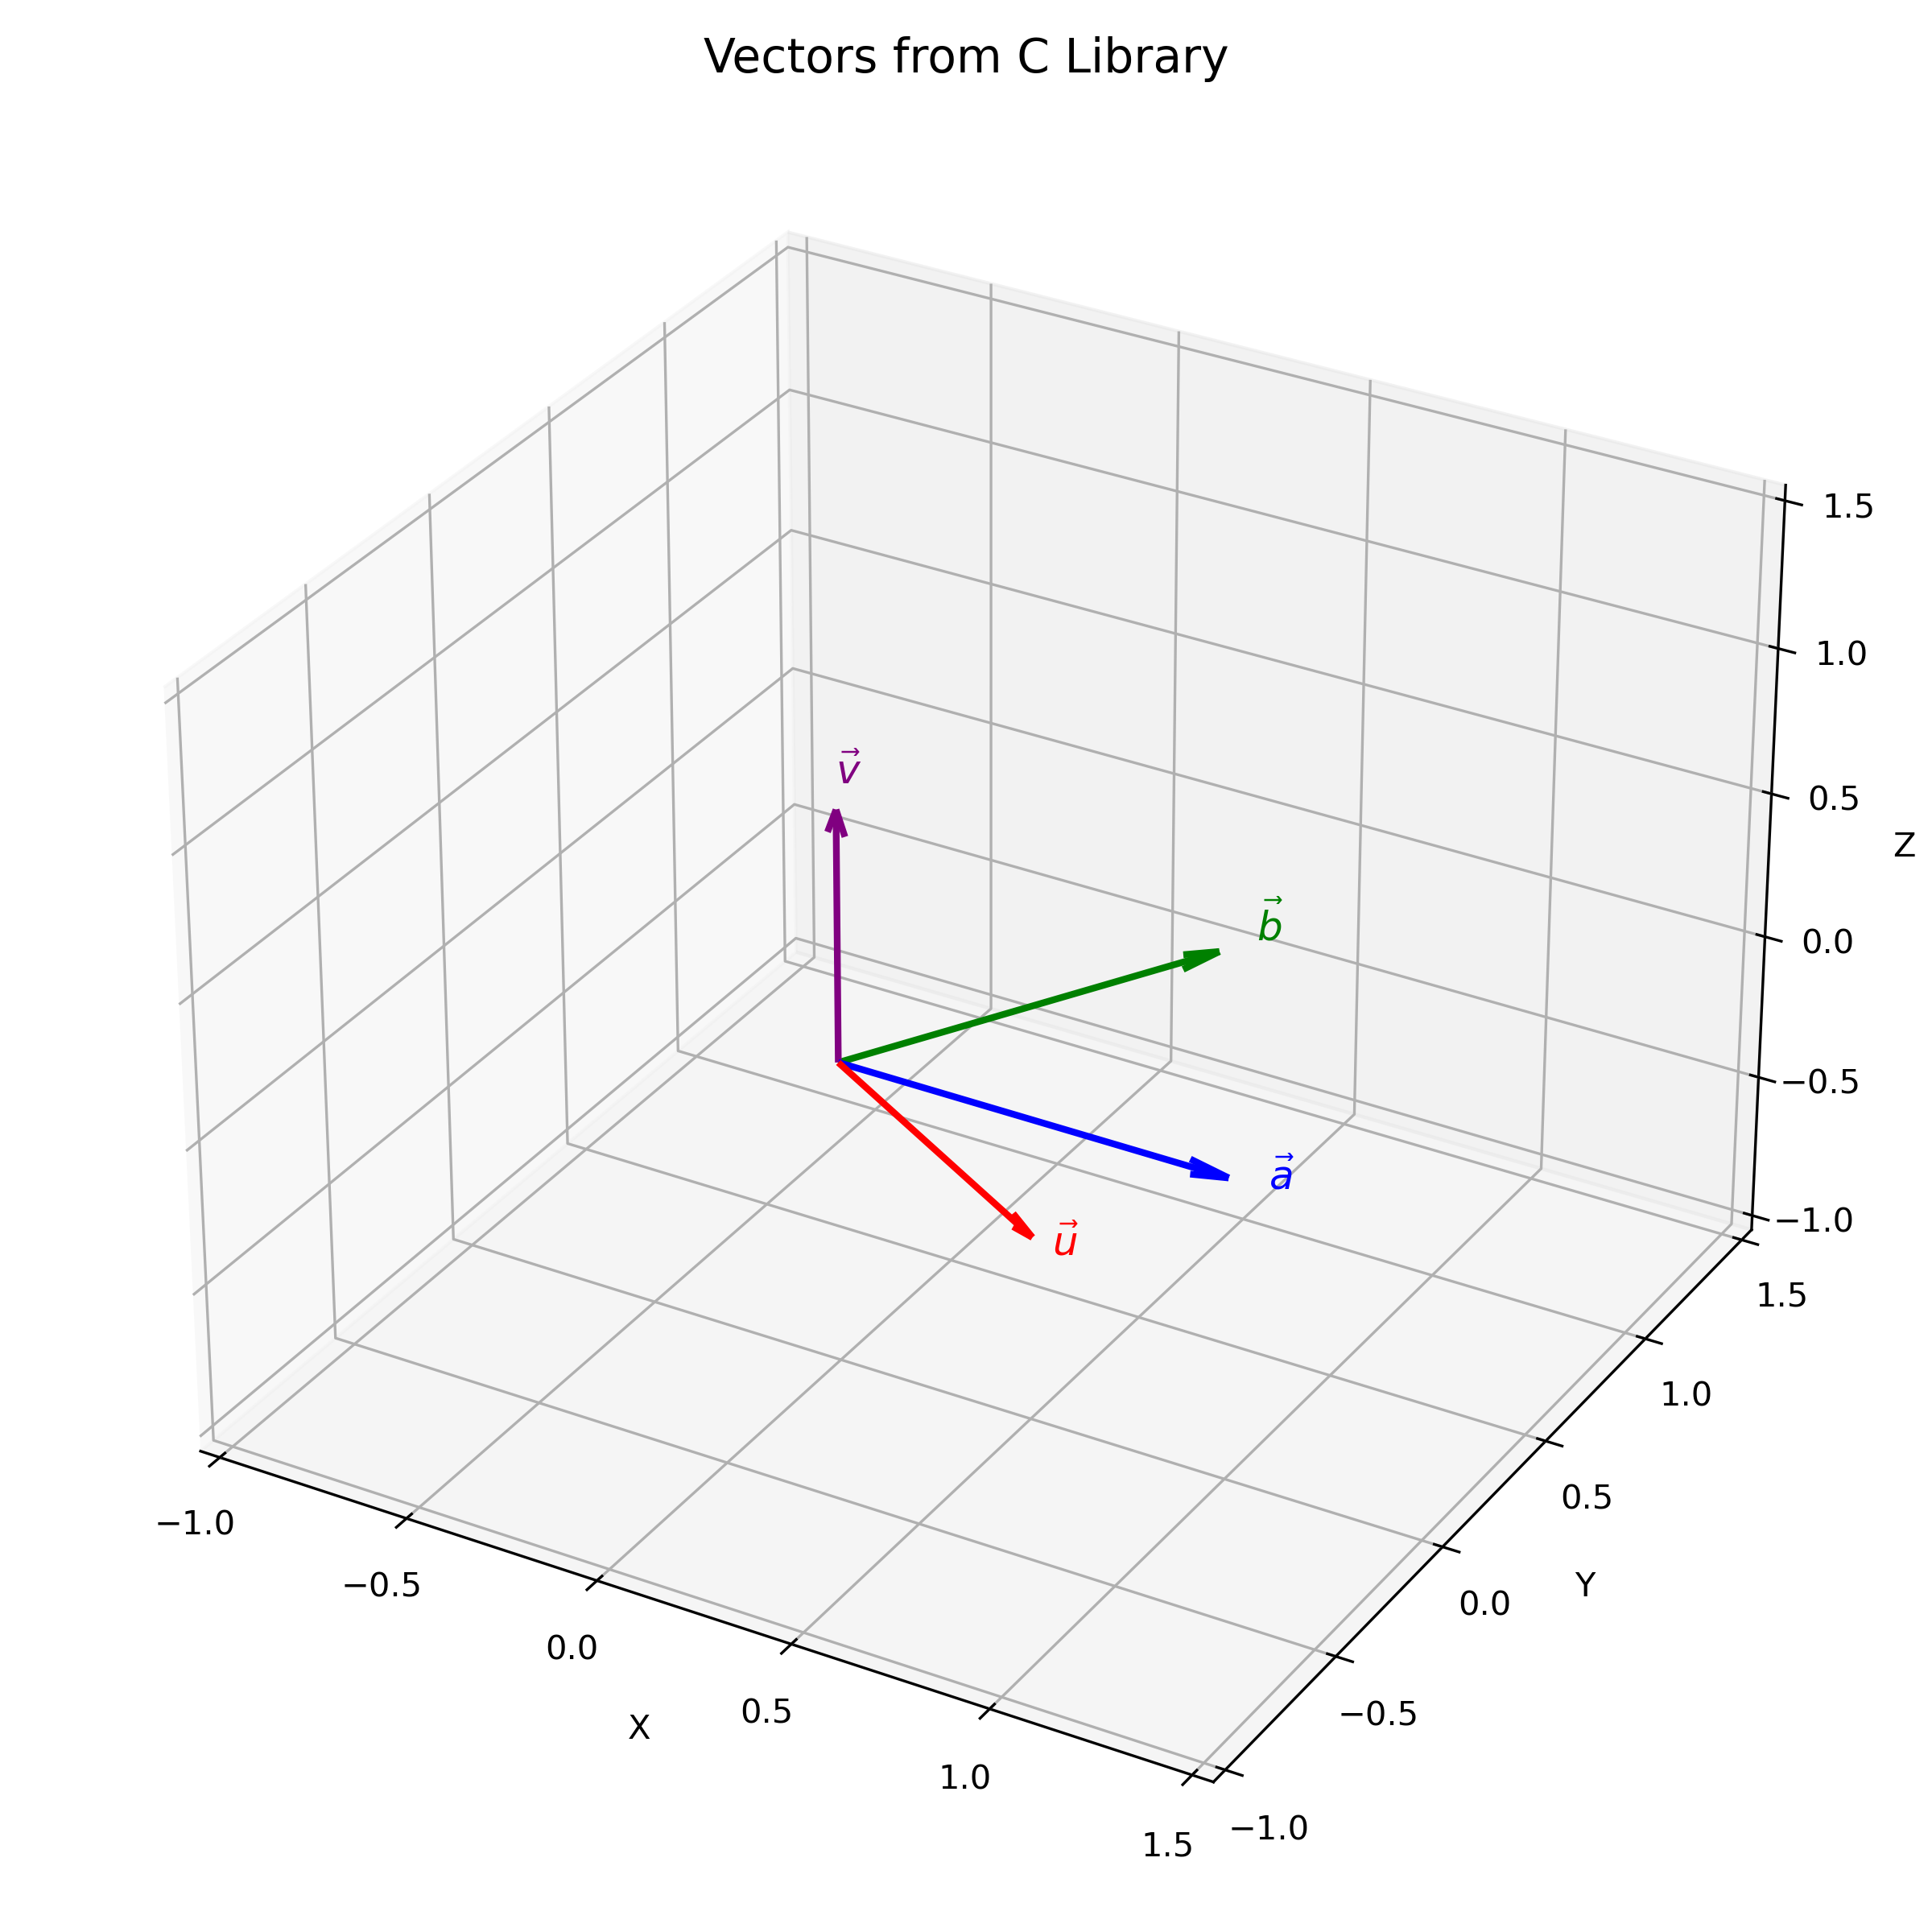
\includegraphics[width=0.9\columnwidth]{figs/vector_plot.png}
    \caption{}
    \label{fig:placeholder}
\end{figure}

\end{document}
